\documentclass[aspectratio=169,11pt]{beamer}
\usepackage[utf8]{inputenc}
\usepackage[T1]{fontenc}
\usepackage[brazilian]{babel}
\usepackage{graphicx,array,tikz,alltt}
\usetikzlibrary{arrows.meta,positioning,shadows}
\usetheme{Singapore}

% Mesmo design das semanas 1 e 2 (slides/semana-0N/*.tex).
% A figura do fluxo e as capturas da interface sao as da semana 2
% (../semana-02/figs); nada e duplicado aqui.
% Compilar: sh compilar.sh (Linux) ou compilar.ps1 (Windows).
\definecolor{ink}{HTML}{202124}
\definecolor{muted}{HTML}{666666}
\definecolor{blue}{RGB}{30,80,160}
\definecolor{green}{RGB}{30,130,60}
\definecolor{red}{RGB}{190,60,60}
\definecolor{orange}{RGB}{200,110,20}
\definecolor{light}{HTML}{E8E8E8}
\setbeamercolor{normal text}{fg=ink,bg=white}
\setbeamercolor{structure}{fg=blue}
\setbeamersize{text margin left=8mm,text margin right=8mm}
\setbeamertemplate{navigation symbols}{}
\setbeamerfont{framesubtitle}{size=\large}
\setbeamertemplate{footline}[frame number]
\setbeamerfont{page number in head/foot}{size=\small}
\newcommand{\muted}[1]{{\small\color{muted}#1\par}}

% caixa com altura minima (caixas lado a lado ficam iguais), sem hifenizacao
\newcommand{\caixacor}[4]{%   cor, largura, altura minima, texto
  \begin{tikzpicture}
    \node[draw=#1!50,fill=#1!6,rounded corners=3pt,text width=#2,minimum height=#3,
          inner sep=8pt,align=left,
          execute at begin node={\hyphenpenalty=10000\exhyphenpenalty=10000}] {#4};
  \end{tikzpicture}}
\newcommand{\caixaalta}[3]{\caixacor{blue}{#1}{#2}{#3}}
\newcommand{\caixa}[2]{\caixaalta{#1}{0pt}{#2}}

% cartao de resultado, com faixa de titulo (como na semana 2)
\newcommand{\resultado}[3]{%
  \begin{tikzpicture}[baseline=0pt]
    \def\L{4.25cm}\def\A{5cm}
    \draw[draw=blue!40,fill=blue!5,rounded corners=4pt] (0,0) rectangle (\L,-\A);
    \fill[blue,rounded corners=4pt] (0,0) rectangle (\L,-9mm);
    \fill[blue] (0,-5mm) rectangle (\L,-9mm);
    \node[text=white,font=\large\bfseries] at (.5*\L,-4.5mm) {#1};
    \node[anchor=north,text width=\L-8mm,align=center] at (.5*\L,-14mm)
      {{\Large\bfseries\color{blue}#2\par}\vspace{3mm}
       {\color{muted}\rule{12mm}{.6pt}\par}\vspace{2mm}
       {\small #3}};
  \end{tikzpicture}}

% caixa de codigo com moldura colorida
\newcommand{\codigo}[2]{%   cor, conteudo (uma lrbox)
  \begin{tikzpicture}
    \node[draw=#1,line width=1pt,fill=#1!5,rounded corners=3pt,inner sep=6pt] {#2};
  \end{tikzpicture}}

% um dos modelos de regra: cor, largura, titulo, exemplo
\newcommand{\modelo}[4]{\caixacor{#1}{#2}{27mm}{{\small\color{#1}\bfseries #3\par}\vspace{1mm}{\small #4}}}

\title[Pré-apresentação]{Regras da equipe sem escrever PDDL}
\author[Grupo B]{Luis Junior \and Manuela Dalmonte \and Vítor Feijó}
\date{INF99003 -- Ciclo 3 -- Grupo B\\Semana 4 | Pré-apresentação}
\hypersetup{pdfauthor={Luis Junior; Manuela Dalmonte; Vítor Feijó}}

\begin{document}

% 1 — Capa.
\begin{frame}[c]
  \titlepage
\end{frame}

\section{Onde estamos}
% 2 — Situacao do projeto e do relatorio, a uma semana da entrega.
\newcommand{\estado}[4]{\caixacor{#1}{.27\textwidth}{49mm}{%
  {\normalsize\color{#1}\bfseries #2\par}\vspace{2mm}{\small #3\par}}}
\begin{frame}{A uma semana da entrega}
  \centering
  \estado{green}{Pronto no relatório}{%
    Contexto e problema\\
    Hipóteses H1 a H3\\
    Implementação do compilador\\
    Projeto experimental\\
    Resultados de H1 a H3\\
    Impacto e conclusões\\
    Guia de reprodutibilidade}{}\hfill
  \estado{orange}{Feito no código, falta no texto}{%
    Alternativas (``ou'')\\
    Restrições de horário e dois turnos\\
    Tradução de regras por modelo de linguagem\\[2mm]
    {\color{muted}Entram no resumo, na implementação e nos créditos.}}{}\hfill
  \estado{red}{Falta}{%
    Avaliar a tradução por modelo de linguagem (H4)\\
    Título e dados dos autores\\
    Revisão final do relatório\\
    Ensaio da apresentação final}{}\par
  \vspace{4mm}
  \muted{Hoje: o relatório, na ordem das suas seções. Entrega e apresentação final: 04/12.}
\end{frame}

\section{Problema}
% 3 — Contexto e problema (secao 1 do relatorio).
\begin{frame}{O problema}
  \begin{columns}[T,onlytextwidth]
    \column{.32\textwidth}
    \centering
    \caixaalta{.92\textwidth}{34mm}{\textbf{A lei}\\Aferir pressão e medir glicemia exigem curso técnico, equipamento e supervisão (Lei 11.350/2006)}
    \column{.32\textwidth}
    \centering
    \caixaalta{.92\textwidth}{34mm}{\textbf{Os materiais}\\Insumos finitos, repostos só na Unidade Básica de Saúde}
    \column{.32\textwidth}
    \centering
    \caixaalta{.92\textwidth}{34mm}{\textbf{A equipe}\\Regras próprias: higienizar as mãos, N95 na suspeita de tuberculose}
  \end{columns}
  \vspace{5mm}
  \centering
  \caixacor{red}{.94\textwidth}{0pt}{\centering\large Modelado em \textbf{PDDL}, cada regra nova exige editar o domínio em vários pontos: só quem programa consegue.}\par
  \vspace{3mm}
  \muted{Dados sintéticos: 10 pacientes fictícios. Só as coordenadas são reais.}
\end{frame}

\section{Solução}
% 4 — A solucao: fluxo da interface ao planejador (figura da semana 2).
\begin{frame}[c]{A solução}
  \centering
  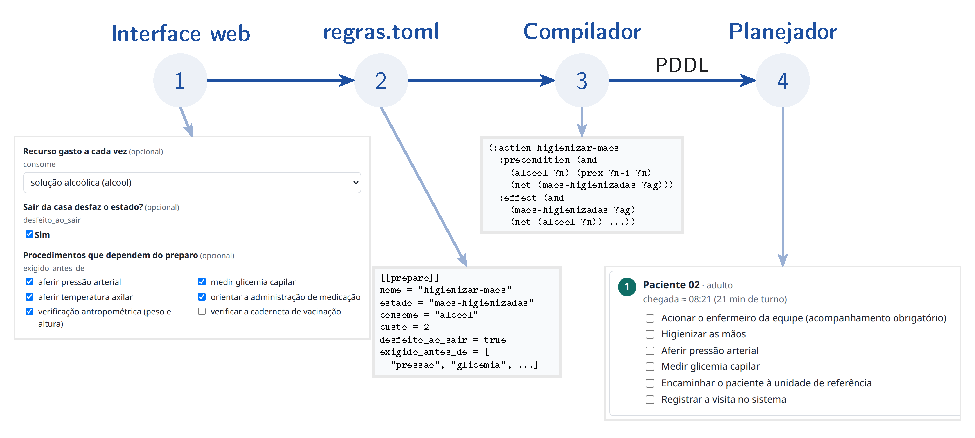
\includegraphics[width=.96\textwidth]{../semana-02/figs/01-compilador.pdf}\par
  \muted{O compilador é determinístico, sem IA. A lei fica travada: as regras só acrescentam exigências.}
\end{frame}

% 5 — Hipoteses (secao 2).
\renewcommand{\arraystretch}{1.55}
\begin{frame}{Hipóteses e métricas}
  \small
  \begin{tabular}{@{}>{\bfseries\color{blue}}p{7mm}p{.34\textwidth}p{.29\textwidth}p{.17\textwidth}@{}}
    $H_1$ & Regras nos modelos, compiladas, equivalem ao PDDL escrito à mão
          & Mesma estrutura e mesmo custo ótimo em cada instância
          & {\color{green}\bfseries Confirmada}\\
    $H_2$ & Descrever a regra exige menos linhas que alterar o PDDL
          & Linhas de TOML contra linhas de PDDL alteradas
          & {\color{green}\bfseries Confirmada}\\
    $H_3$ & Com as regras ativas, o roteiro de 10 pacientes sai em até 120\,s por busca
          & Acréscimo em minutos ao turno ótimo e tempo até o roteiro
          & {\color{green}\bfseries Confirmada}\\
    $H_4$ & Alternativas e horários cabem nos modelos, e um modelo de linguagem traduz regras
          & Proporção das regras geradas que compilam e coincidem com um gabarito
          & {\color{orange}\bfseries Em avaliação}\\
  \end{tabular}
\end{frame}

\section{Implementação}
% 6 — Os modelos fixos: cinco da semana 2 e dois novos.
\begin{frame}{Sete modelos fixos}
  \centering
  \modelo{blue}{.20\textwidth}{A. Recurso}{6 doses de álcool, repostas na UBS}\hfill
  \modelo{blue}{.20\textwidth}{B. Preparo}{Higienizar as mãos}\hfill
  \modelo{blue}{.20\textwidth}{C. Pré-requisito}{Higienizar antes de aferir a pressão}\hfill
  \modelo{blue}{.20\textwidth}{D. Consumo}{Cada glicemia gasta 2 algodões}\par
  \vspace{3mm}
  \modelo{blue}{.26\textwidth}{E. Exigência}{Suspeita de tuberculose exige N95 (por paciente)}\hfill
  \modelo{green}{.26\textwidth}{F. Alternativa (OU)}{Um de dois preparos antes da medição}\hfill
  \modelo{green}{.26\textwidth}{G. Período}{Gestantes só de manhã}\par
  \vspace{3mm}
  \muted{Em verde, os modelos novos. O que não cabe nos modelos fica de fora, em vez de virar um PDDL que ninguém consegue conferir.}
\end{frame}

% 7 — Pipeline e algoritmos (secao 3).
\newcommand{\etapa}[2]{\node[draw=blue!50,fill=blue!6,rounded corners=3pt,minimum height=9mm,
  text width=19mm,align=center,font=\footnotesize,inner sep=2pt] (#1) {#2};}
\begin{frame}{O que acontece por baixo}
  \centering
  \begin{tikzpicture}[node distance=4mm,flow/.style={-{Stealth[length=2mm]},draw=blue!55,line width=.7pt}]
    \etapa{a}{Seleção}
    \node[draw=blue!50,fill=blue!6,rounded corners=3pt,minimum height=9mm,text width=19mm,
          align=center,font=\footnotesize,inner sep=2pt,right=of a] (b) {Rota};
    \node[draw=blue!50,fill=blue!6,rounded corners=3pt,minimum height=9mm,text width=19mm,
          align=center,font=\footnotesize,inner sep=2pt,right=of b] (c) {Compilação};
    \node[draw=blue!50,fill=blue!6,rounded corners=3pt,minimum height=9mm,text width=19mm,
          align=center,font=\footnotesize,inner sep=2pt,right=of c] (d) {Busca};
    \node[draw=blue!50,fill=blue!6,rounded corners=3pt,minimum height=9mm,text width=19mm,
          align=center,font=\footnotesize,inner sep=2pt,right=of d] (e) {Limpeza};
    \node[draw=blue!50,fill=blue!6,rounded corners=3pt,minimum height=9mm,text width=19mm,
          align=center,font=\footnotesize,inner sep=2pt,right=of e] (f) {Roteiro};
    \draw[flow] (a) -- (b); \draw[flow] (b) -- (c); \draw[flow] (c) -- (d);
    \draw[flow] (d) -- (e); \draw[flow] (e) -- (f);
  \end{tikzpicture}\par
  \muted{A rota usa o vizinho mais próximo com 2-opt. As regras entram na compilação, sobre o domínio legal.}
  \vspace{2mm}
  \begin{columns}[T,onlytextwidth]
    \column{.32\textwidth}
    \centering
    \caixaalta{.92\textwidth}{40mm}{\textbf{Instanciação com poda}\\Descarta a combinação assim que uma precondição fixa falha\\[2mm]{\color{blue}\bfseries 4,7 bilhões $\rightarrow$ 9.449 ações}}
    \column{.32\textwidth}
    \centering
    \caixaalta{.92\textwidth}{40mm}{\textbf{Busca}\\Fast Downward com LM-cut, ou A* com $h_{max}$\\[2mm]{\color{blue}\bfseries Janelas: ótimo nas próximas $k=3$ visitas, avançando uma}}
    \column{.32\textwidth}
    \centering
    \caixaalta{.92\textwidth}{40mm}{\textbf{Limpeza}\\Remove ações redundantes do plano\\[2mm]{\color{blue}\bfseries Nunca aumenta o custo}}
  \end{columns}
\end{frame}

\section{Experimentos}
% 8 — Projeto experimental (secao 4).
\begin{frame}{Como avaliamos}
  \begin{columns}[T,onlytextwidth]
    \column{.48\textwidth}
    \centering
    \caixaalta{.94\textwidth}{31mm}{\textbf{Equivalência ($H_1$)}\\24 instâncias de 2 a 4 pacientes, com capacidades reduzidas para forçar reposições. Controle negativo: 8 alterações propositais nas regras}\par
    \vspace{2mm}
    \caixaalta{.94\textwidth}{31mm}{\textbf{Medições ($H_2$ e $H_3$)}\\Sete regras novas (R1 a R7), sozinhas e acumuladas, de 1 a 10 pacientes. Cada configuração roda uma vez: o resultado é determinístico}
    \column{.48\textwidth}
    \centering
    \caixaalta{.94\textwidth}{31mm}{\textbf{Variáveis}\\Regras ativas, nº de pacientes, estratégia de busca. Medimos linhas, custo do turno (min), ações instanciadas e tempo. Mesma planilha e mesma rota, limite de 120\,s}\par
    \vspace{2mm}
    \caixaalta{.94\textwidth}{31mm}{\textbf{Ambiente}\\Core Ultra 5 245KF, 16\,GB, Windows 11, Python 3.14 e Fast Downward. Tudo reproduzível com \texttt{python acs.py}}
  \end{columns}
\end{frame}

\section{Resultados}
% 9 — H1: correcao.
\begin{frame}{$H_1$: o compilador está correto}
  \centering
  \resultado{Estrutura}{Igual}{parâmetros, precondições, efeitos e custo das ações}\hfill
  \resultado{Comportamento}{24 de 24}{instâncias com o mesmo custo ótimo nos dois domínios}\hfill
  \resultado{Controle negativo}{8 de 8}{alterações propositais acusadas pela comparação estrutural}\par
  \vspace{4mm}
  \muted{Três regras do Ciclo 2 escritas como modelos contra o domínio estendido escrito à mão pelo outro grupo.}
\end{frame}

% 10 — H2: esforco, com grafico de barras (dados da Tabela 1 do relatorio).
\begin{frame}{$H_2$: regras mais curtas que o PDDL}
  \begin{columns}[c,onlytextwidth]
    \column{.66\textwidth}
    \centering
    \begin{tikzpicture}[x=1cm,y=1cm]
      \foreach \i/\vt/\vp/\nm in {0/8/27/lancetas, 1/13/36/termôm., 2/7/13/balança,
                                  3/18/60/avental, 4/18/60/N95, 5/17/52/luvas, 6/12/41/algodão}{
        \fill[blue!75] ({\i*1.28},0) rectangle ({\i*1.28+.4},{\vt*.055});
        \fill[orange!85] ({\i*1.28+.44},0) rectangle ({\i*1.28+.84},{\vp*.055});
        \node[above,font=\tiny] at ({\i*1.28+.2},{\vt*.055}) {\vt};
        \node[above,font=\tiny] at ({\i*1.28+.64},{\vp*.055}) {\vp};
        \node[below,font=\scriptsize] at ({\i*1.28+.42},0) {\nm};
      }
      \draw[muted,line width=.5pt] (-.2,0) -- (8.5,0);
      \fill[blue!75] (0,3.9) rectangle ++(.3,.2);
      \node[right,font=\small] at (.35,4.0) {TOML escrito};
      \fill[orange!85] (2.6,3.9) rectangle ++(.3,.2);
      \node[right,font=\small] at (2.95,4.0) {PDDL alterado};
    \end{tikzpicture}\par
    \muted{Linhas por regra (R1 a R7), sem comentários.}
    \column{.31\textwidth}
    \centering
    \caixaalta{.95\textwidth}{0pt}{\centering{\Large\bfseries\color{blue}3,1\par}\vspace{1mm}linhas de PDDL evitadas, em média, por cada linha de TOML}\par
    \vspace{3mm}
    \caixaalta{.95\textwidth}{0pt}{\centering{\Large\bfseries\color{blue}7 a 18\par}\vspace{1mm}linhas de TOML contra 13 a 60 de PDDL}
  \end{columns}
\end{frame}

% 11 — H3: viabilidade e escala.
\begin{frame}{$H_3$: o roteiro sai, mas o ótimo não escala}
  \centering
  \resultado{Barato}{+1 a 9 min}{por regra, num turno ótimo de 386 min}\hfill
  \resultado{Rápido}{0,2 s}{para o primeiro plano do Fast Downward, em todos os casos}\hfill
  \resultado{Ótimo difícil}{$>$ 120 s}{a partir de cinco regras acumuladas; até quatro, 31 s}\par
  \vspace{3mm}
  \muted{Com as sete regras e 10 pacientes, as janelas dão 430 min em 16\,s. O planejador do Ciclo 2 sozinho não termina a partir de seis regras.}
\end{frame}

% 12 — Extensoes (hipotese H4): OU, turnos e traducao por modelo de linguagem.
\newsavebox{\codealt}
\newsavebox{\codeper}
\begin{frame}[fragile]{Extensões: ou, horários e tradução}
\begin{lrbox}{\codealt}\begin{minipage}{6.1cm}\scriptsize
\begin{alltt}
[[alternativa]]
nome = "conferencia-do-aparelho"
preparos = ["conferir-aparelho",
            "conferir-kit"]
antes_de = ["pressao"]
\end{alltt}
\end{minipage}\end{lrbox}%
\begin{lrbox}{\codeper}\begin{minipage}{6.1cm}\scriptsize
\begin{alltt}
[[periodo]]
nome = "gestantes-pela-manha"
marca = "gestante"
turnos = ["manha"]
\end{alltt}
\end{minipage}\end{lrbox}%
  \begin{columns}[T,onlytextwidth]
    \column{.50\textwidth}
    \centering
    {\color{green}\bfseries Duas regras novas e dois turnos\par}
    \vspace{.5mm}
    \codigo{green}{\usebox{\codealt}}\par
    \vspace{2mm}
    \codigo{green}{\usebox{\codeper}}\par
    \column{.46\textwidth}
    \centering
    {\color{blue}\bfseries Tradução por modelo de linguagem\par}
    \vspace{.5mm}
    \caixa{.94\textwidth}{\small ``Pacientes marcados como gestante só podem ser visitados pela manhã''}\par
    \vspace{.5mm}
    {\color{blue}$\downarrow$}\par
    \caixa{.94\textwidth}{\small Blocos candidatos, conferidos pelo compilador}\par
    \vspace{.5mm}
    {\color{blue}$\downarrow$}\par
    \caixa{.94\textwidth}{\small A equipe revisa e edita no formulário}\par
  \end{columns}
  \vspace{1mm}
  \centering
  \caixacor{orange}{.94\textwidth}{0pt}{\centering\footnotesize Implementado e testado. {\bfseries A avaliação de $H_4$ ainda falta:} quantas regras geradas compilam e coincidem com o gabarito.}
\end{frame}

\section{Impacto}
% 13 — Impacto e transferencia tecnologica (secao 5).
\begin{frame}{Impacto e caminho até o uso}
  \begin{columns}[T,onlytextwidth]
    \column{.48\textwidth}
    \centering
    {\large\color{blue}Impacto\par}
    \vspace{2mm}
    \caixaalta{.94\textwidth}{19mm}{\textbf{Social}\\A equipe mantém as próprias regras, sem depender de quem programa}\par
    \vspace{1.5mm}
    \caixaalta{.94\textwidth}{19mm}{\textbf{Econômico}\\Cada regra mostra seu custo (1 a 9 min) antes de ser adotada}\par
    \vspace{1.5mm}
    \caixaalta{.94\textwidth}{19mm}{\textbf{LGPD}\\Dados fictícios, execução local, e a tradução só recebe o texto da regra}
    \column{.48\textwidth}
    \centering
    {\large\color{blue}Transferência\par}
    \vspace{2mm}
    \caixaalta{.94\textwidth}{19mm}{\textbf{Parceiros}\\Secretarias municipais de saúde e o e-SUS Território}\par
    \vspace{1.5mm}
    \caixaalta{.94\textwidth}{19mm}{\textbf{Maturidade}\\Entre os níveis 3 e 4: protótipo validado em laboratório}\par
    \vspace{1.5mm}
    \caixaalta{.94\textwidth}{19mm}{\textbf{Falta para produção}\\Cadastro do e-SUS, distâncias pelas ruas e uso sem conexão}
  \end{columns}
\end{frame}

\section{Conclusões}
% 14 — Limites e licoes (secao 6).
\begin{frame}{O que aprendemos}
  \begin{columns}[T,onlytextwidth]
    \column{.48\textwidth}
    \centering
    {\large\color{red}O que foi refutado\par}
    \vspace{2mm}
    \caixacor{red}{.94\textwidth}{40mm}{Nossa tese inicial: o planejamento acharia planos que um programa comum não acha.\\[2mm]Corrigido, o programa procedural acha os mesmos planos.}\par
    \vspace{1.5mm}
    {\small A tese que se sustentou é o custo de manutenção: o PDDL se adapta a regras novas sem mudar código.\par}
    \column{.48\textwidth}
    \centering
    {\large\color{blue}Limites\par}
    \vspace{2mm}
    \caixaalta{.94\textwidth}{9mm}{O ótimo com muitas regras é desconhecido; o plano das janelas está cerca de 5\% acima, por estimativa}\par
    \vspace{1.5mm}
    \caixaalta{.94\textwidth}{9mm}{A rota é escolhida só pela distância, sem considerar as regras}\par
    \vspace{1.5mm}
    \caixaalta{.94\textwidth}{9mm}{Dados sintéticos, e cada configuração foi executada uma vez}
  \end{columns}
\end{frame}

\section{Próximos passos}
% 15 — O que falta ate 04/12.
\begin{frame}{Até 04/12}
  \begin{columns}[T,onlytextwidth]
    \column{.48\textwidth}
    \centering
    {\large\color{blue}Relatório\par}
    \vspace{3mm}
    \caixaalta{.94\textwidth}{17mm}{\textbf{Avaliar $H_4$}\\Descrições de regras com gabarito, no modelo de linguagem}\par
    \vspace{2mm}
    \caixaalta{.94\textwidth}{17mm}{\textbf{Atualizar o texto}\\Resumo, implementação, resultados e créditos com as extensões}\par
    \column{.48\textwidth}
    \centering
    {\large\color{blue}Entrega\par}
    \vspace{3mm}
    \caixaalta{.94\textwidth}{17mm}{\textbf{Fechar pendências}\\Título, dados dos autores e revisão final}\par
    \vspace{2mm}
    \caixaalta{.94\textwidth}{17mm}{\textbf{Apresentação final}\\Ensaio e demonstração na interface}\par
  \end{columns}
\end{frame}

% 16 — Creditos, como nas semanas 1 e 2.
\begin{frame}{Encerramento e créditos}
  \centering
  {\large Obrigado pela participação!\par}
  \vspace{9mm}
  \begin{columns}[T,onlytextwidth]
    \column{.48\textwidth}
    \centering
    {\large\color{blue}Projeto original\par}
    \vspace{2mm}
    \textbf{Grupo B -- Ciclo 2}\par
    \vspace{4mm}
    Gabriel Knopp\par
    Arthur Silva\par
    Izadora Oliveira
    \column{.48\textwidth}
    \centering
    {\large\color{blue}Compilador e interface\par}
    \vspace{2mm}
    \textbf{Grupo B -- Ciclo 3}\par
    \vspace{4mm}
    Luis Junior\par
    Manuela Dalmonte\par
    Vítor Feijó
  \end{columns}
\end{frame}

\end{document}
